\documentclass[10pt, aspectratio=169]{beamer}

\newcommand{\templates}{cel-slides}

\input{\templates/packages.tex}
\input{\templates/KITColors.tex}
\usepackage{mathtools}
\usepackage{stmaryrd}
\usepackage{braket}
\providecolor{KITblack}{RGB}{0,0,0}
\definecolor{myred}{RGB}{202,0,32}

% Template switches
\newbool{space_for_face}
\boolfalse{space_for_face}
\newbool{small_subitems}
\boolfalse{small_subitems}
\newbool{hide_author_in_footer}
\booltrue{hide_author_in_footer}
\newbool{cel_on_title}
\booltrue{cel_on_title}
\newbool{erc_on_title}
\booltrue{erc_on_title}
\newbool{dfg_on_title}
\boolfalse{dfg_on_title}
\newbool{bmbf_on_title}
\boolfalse{bmbf_on_title}
\newbool{bmftr_on_title}
\booltrue{bmftr_on_title}
\newbool{bmwk_on_title}
\boolfalse{bmwk_on_title}
\newbool{bmwi_on_title}
\boolfalse{bmwi_on_title}
\newbool{use_real_footnotesize}
\booltrue{use_real_footnotesize}
\newbool{overview_at_subsection}
\boolfalse{overview_at_subsection}
\newbool{first_overview_unshaded}
\booltrue{first_overview_unshaded}
\newbool{use_legacy_citations}
\booltrue{use_legacy_citations}
\newbool{EnglishLanguage}
\booltrue{EnglishLanguage}

\input{\templates/modifications.tex}
\input{\templates/makros_own.tex}

\usetikzlibrary{decorations.pathreplacing,fit,positioning}
\pgfplotsset{compat=1.18}

% A compact frame title avoids collisions with dense technical slides.
\setbeamertemplate{frametitle}
{
  \begin{textblock*}{135mm}(6mm,4mm)
    {\bfseries\usebeamerfont{frametitle}\textcolor{black}{\LARGE\insertframetitle}}
  \end{textblock*}
  \begin{textblock*}{15mm}(146mm,4mm)
    \iflanguage{english}{%
      \includegraphics[width=18mm]{\templates/logos/kitlogo_en_rgb}
    }{%
      \includegraphics[width=18mm]{\templates/logos/kitlogo_de_rgb}
    }%
  \end{textblock*}
  \vspace{1.05cm}
}

\setbeamerfont{caption}{size=\scriptsize}
\setbeamerfont{footnote}{size=\tiny}

% Local notation
\newcommand{\bH}{\mathbf{H}}
\newcommand{\bP}{\mathbf{P}}
\newcommand{\bD}{\mathbf{D}}
\newcommand{\bM}{\mathbf{M}}
\newcommand{\bS}{\mathbf{S}}
\newcommand{\bA}{\mathbf{A}}
\newcommand{\bB}{\mathbf{B}}
\newcommand{\bI}{\mathbf{I}}
\newcommand{\bone}{\mathbf{1}}
\newcommand{\bzero}{\mathbf{0}}
\newcommand{\br}{\mathbf{r}}
\newcommand{\be}{\mathbf{e}}
\newcommand{\bz}{\mathbf{z}}
\newcommand{\Ftwo}{\mathbb{F}_{2}}
\newcommand{\Fq}{\mathbb{F}_{2^\ell}}
\newcommand{\CAMEL}{\textsc{CAMEL}}
\newcommand{\DPM}{DPM}
\newcommand{\QD}{QD}
\newcommand{\BPfour}{BP4}
\newcommand{\baromega}{\bar{\omega}}
\newcommand{\I}{\bm{I}}
\newcommand{\X}{\textcolor{KITblue}{\bm{X}}}
\newcommand{\Z}{\textcolor{KITorange}{\bm{Z}}}
\newcommand{\Y}{\textcolor{KITred}{\bm{Y}}}
\newcommand{\If}{0}
\newcommand{\Xf}{\textcolor{KITblue}{\omega}}
\newcommand{\Zf}{\textcolor{KITorange}{\baromega}}
\newcommand{\Yf}{\textcolor{KITred}{1}}
\newcommand{\codeparams}[2]{\llbracket #1,#2\rrbracket}
\newcommand{\tinycite}[1]{\textcolor{KITblack!70}{\scriptsize #1}}
\newcommand{\dyadicAblock}[1]{\textcolor{myred}{#1}}
\newcommand{\dyadicBblock}[1]{\textcolor{KITblue}{#1}}
\newcommand{\dyadicfour}[4]{%
  \begin{pmatrix}
    \dyadicAblock{#1} & \dyadicAblock{#2} & \dyadicBblock{#3} & \dyadicBblock{#4}\\
    \dyadicAblock{#2} & \dyadicAblock{#1} & \dyadicBblock{#4} & \dyadicBblock{#3}\\
    \dyadicBblock{#3} & \dyadicBblock{#4} & \dyadicAblock{#1} & \dyadicAblock{#2}\\
    \dyadicBblock{#4} & \dyadicBblock{#3} & \dyadicAblock{#2} & \dyadicAblock{#1}
  \end{pmatrix}}
\newcommand{\DtwoExampleMatrix}{%
  \begin{pmatrix}
    0&0&1&0&0&0&0&0\\
    0&0&0&1&0&0&0&0\\
    1&0&0&0&0&0&0&0\\
    0&1&0&0&0&0&0&0\\
    0&0&0&0&0&0&1&0\\
    0&0&0&0&0&0&0&1\\
    0&0&0&0&1&0&0&0\\
    0&0&0&0&0&1&0&0
  \end{pmatrix}}

\title[Sisi Miao: CSS QLDPC Codes based on Dyadic Matrices]{Quantum CSS LDPC Codes based on Dyadic Matrices for \\ Belief Propagation-based Decoding}
\author[Sisi Miao]{\texorpdfstring{Alessio Baldelli$^\dagger$,
Massimo Battaglioni$^\dagger$,
Jonathan Mandelbaum$^\star$,
\underline{Sisi Miao}$^\star$,
Laurent Schmalen$^\star$\\
\footnotesize $^\dagger$\, \emph{Department of Information Engineering}, Universit\`a Politecnica delle Marche, Ancona 60131, Italy\\
$^\star$\,\emph{Communications Engineering Lab (CEL)}, Karlsruhe Institute of Technology (KIT), 76187 Karlsruhe, Germany}{Alessio Baldelli, Massimo Battaglioni, Jonathan Mandelbaum, Sisi Miao, Laurent Schmalen}}
\institute{Karlsruhe Institute of Technology (KIT), Communications Engineering Lab (CEL)}
%\date{ISIT 2026}

\usepackage{makecell}
\begin{document}
\selectlanguage{english}

\begin{frame}[plain]
  \maketitle
\end{frame}


\begin{frame}[c]{Background}
    \begin{columns}
        \begin{column}{0.6\textwidth}
            \onslide<1->{\begin{itemize}
                             \item Quantum error-correcting codes are crucial for realizing quantum computers
                             \item \schlagwort{Quantum LDPC (QLDPC) codes} are promising candidates
                             \item Belief propagation (BP) is the native decoder for LDPC codes
                             \item In principle, \schlagwort{quaternary BP (BP4)} can be used to decode QLDPC codes
                             \begin{itemize}
                                 \item Map 4 Pauli errors $\{\I,\X,\Z,\Y\}$ into GF(4) elements $\{\If,\Xf,\Zf,\Yf\}$
                                 \item E.g., $\I\mapsto \If,\X \mapsto \Xf,\Z\mapsto \Zf,\Y\mapsto \Yf$
                             \end{itemize}
                             \item However, BP4 for QLDPC codes often yields poor performance
            \end{itemize}}
        \end{column}

        \begin{column}{0.4\textwidth}
            \onslide<2>{
                \vspace{1cm}


                \centering \phantom{xxxxxxxx} $\llbracket 72,2,6 \rrbracket$ toric code~\citereference{Kit03}

                \vspace{-0.4cm}

                \begin{center}
                    \begin{tikzpicture}
\pgfplotsset{grid style={gray!70}}
\pgfplotsset{every tick label/.append style={font=\footnotesize}}
\begin{axis}[%
    scale only axis=true,
    width=4cm,
    height=3.5cm,
    xmin=0.015,
    xmax=0.15,
    % xmode=log,
    ymode=log,
    ymin=1e-5,
    ymax=1,
    yminorticks,
    axis background/.style={fill=white, mark size=1.5pt},
    xminorticks,
    %ymajorgrids,
    %yminorgrids,
    xtick={0.015,0.045,...,0.15},
    x tick label style={
        /pgf/number format/.cd,
        % using `fixed relative' would normally work ...
        fixed relative,
        precision=3,
    },
%    ytick={1,0.1,0.01,0.001,1e-4,1e-5,1e-6,1e-7,1e-8},
    ylabel={Logical error rate}, xmajorgrids,  ymajorgrids,
    xlabel={Physical error rate $p$},
    label style={font=\small},
    legend cell align={left},
    legend style={at={(1 ,0)},anchor=south east,fill opacity=1, text opacity = 1,legend columns=1,font=\footnotesize}
    ]


     \addplot [color=myred,line width=1pt,mark=o, mark options={solid,myred, mark size=1.9pt}]table[row sep=crcr]{
% [[72,2]], 70 checks, 25 iter, ep0=0.1, not trained
% FE 3061, total dec. 4223\\
0.15 0.72484\\
% FE 3058, total dec. 4781\\
0.135 0.639615\\
% FE 3041, total dec. 5533\\
0.12 0.549611\\
% FE 3028, total dec. 6844\\
0.105 0.442431\\
% FE 3026, total dec. 8536\\
0.09 0.354499\\
% FE 3010, total dec. 11957\\
0.075 0.251735\\
% FE 3018, total dec. 17595\\
0.06 0.171526\\
% FE 3006, total dec. 29874\\
0.045 0.100623\\
% FE 3004, total dec. 67096\\
0.03 0.0447717\\
% FE 1130, total dec. 100000\\
% FE 2220, total dec. 200000\\
% FE 3002, total dec. 268603\\
0.015 0.0111763\\
    };
 \addlegendentry{BP4}
  

  
  \addplot [color=black, dotted,line width=1.5pt,mark=none]table[row sep=crcr]{
0.015 0.00017123287671232877\\
0.031875 0.0020348837209302325\\
0.04875 0.009116883116883117\\
0.065625 0.024413793103448277\\
0.08250000000000002 0.05071428571428571\\
0.099375 0.098\\
0.11624999999999999 0.1478\\
0.13312500000000002 0.201\\
0.15000000000000002 0.275\\
  };
\addlegendentry{MWPM~\citereference{Edm65}}


  
  \addplot [color=black, line width=1pt,mark=none]table[row sep=crcr]{
0.015 0.029775\\
0.03 0.0591\\
0.045 0.087975\\
0.06 0.1164\\
0.075 0.14437\\
0.09 0.1719\\
0.105 0.19898\\
0.12 0.2256\\
0.135 0.25177\\
0.15 0.2775\\
  };
\addlegendentry{uncoded}
    
    % \node[draw, fill=white, anchor = south east] at (axis cs:0.15, 1e-5) {\footnotesize $d=6$};
    \end{axis}
\end{tikzpicture}  

                \end{center}}
        \end{column}
    \end{columns}
    \bigskip
    \bigskip
    \bigskip
    \onslide<2>{
        \addreferences{Kit03}{A. Yu. Kitaev, ``Fault-tolerant quantum computation by anyons,'' \emph{Annals of physics}, 2003.}
        {Edm65}{J. Edmonds, ``Paths, trees, and flowers,'' \emph{Canadian Journal of Mathematics}, 1965}
        \endreferences}
\end{frame}

\begin{frame}[c]{Problem}
\visible<1-2>{
    \begin{itemize}
        \item Short cycles of length 4 are \schlagwort{unavoidable} in the Tanner graph of QLDPC codes
    \end{itemize}
    

            \begin{columns}[T,totalwidth=\linewidth]
                \begin{column}{0.6\linewidth}
                    \begin{itemize}
                        \item \schlagwort{Example}: PCM of an $\llbracket n,k \rrbracket$ CSS-type QLDPC code~\citereference{CRSS98}
                        \vspace{-1ex}
                    \[
                        \bS =
                        \begin{pmatrix}
                            \Xf \bH_X\\
                            \Zf \bH_Z
                        \end{pmatrix}
                    \]
                        \end{itemize}
                \end{column}
                \begin{column}{0.4\linewidth}

                    \resizebox{!}{2.5cm}{\begin{tikzpicture}
\tikzstyle{variable node}=[circle, draw=black, thick,  inner sep=0pt, minimum size=2.4mm]
\tikzstyle{check node}=[rectangle, draw=black, thick, inner sep=0pt, minimum size=2.4mm]        
\tikzstyle{xline} = [draw=KITblue,thick]       
\tikzstyle{zline} = [draw=KITorange,thick,dashed,dash pattern=on 2pt off 1pt]       

\foreach \x in {1,2,...,7}
\node[variable node] (vn\x) at (0, 0.3+6-0.7*\x) [label=left:$\mathsf{v}_{\x}$]{};

\foreach \x in {1,2,...,6}
\node[check node] (cn\x) at (3.5, 0.3+5.6-0.7*\x) [label=right:$\mathsf{c}_{\x}$]{};
% \node at (0, 0) {\footnotesize variable nodes (VN)};
% \node at (3.5, 0) {\footnotesize check nodes (CN)};

\foreach \x in {1,3,5,7}
\path [xline] (cn1) -- (vn\x);
\foreach \x in {2,3,6,7}
\path [xline] (cn2) -- (vn\x);
\foreach \x in {4,5,6,7}
\path [xline] (cn3) -- (vn\x);

\foreach \x in {1,3,5,7}
\path [zline] (cn4) -- (vn\x);
\foreach \x in {2,3,6,7}
\path [zline] (cn5) -- (vn\x);
\foreach \x in {4,5,6,7}
\path [zline] (cn6) -- (vn\x);  
\end{tikzpicture}}
                \end{column}
            \end{columns}
            }
            \vspace{-1cm}
\visible<2>{
            \begin{columns}[c,totalwidth=\linewidth]
                \begin{column}{\linewidth}
                    \begin{itemize}
            \item By construction
            \[
                \bH_X \bH_Z^{\mathsf{T}}
                \overset{\begin{subarray}{c} \text{mod $2$}\end{subarray}}{=}
                \bm{0}
                \Leftrightarrow
                \text{Every row of $\bH_X$ has an even number of overlapping 1s with every row of $\bH_Z$}
            \]
            \item Thus, the rows either have no overlap or form a length-4 cycle, e.g.,
            \[
                \begin{pmatrix}0&0&1&1&0&0\\1&1&0&0&0&0\end{pmatrix}
                \;\;\;\;\;\text{ or }\;\;\;\;\;
                \begin{pmatrix}1&1&0&0&0&0\\1&1&0&0&0&0\end{pmatrix}
            \]
            \item Codes with tree-like Tanner graphs have poor minimum distance~\citereference{ETV99}
        \end{itemize}
        

        \end{column}
    \end{columns}
    }
 \vspace{1em}
      {\scriptsize
    \renewcommand{\arraystretch}{1}
    \begin{tabular}{lp{0.93\textwidth}}
    \visible<1-2>{
      \textcolor{kit-green100}{[CRSS98]}&
      \textcolor{kit-green100}{
        A.~R. Calderbank, E.~M. Rains, P.~W. Shor, and N.~J.~A. Sloane, ``Quantum error correction via codes over \textit{{GF}(4)},'' \emph{TIT}, 1998.
      }\\}
      \visible<2>{
       \textcolor{kit-green100}{[ETV99]} &
      \textcolor{kit-green100}{
        T. Etzion, A. Trachtenberg, and A. Vardy, ``Which codes have cycle-free Tanner graphs?,'' \emph{TIT}, 1999.
      }
      }
    \end{tabular}
  }
  
   
    % \addreferences
    % {CRSS98}{A.~R. Calderbank, E.~M. Rains, P.~W. Shor, and N.~J.~A. Sloane, ``Quantum error correction via codes over \textit{{GF}(4)},'' \emph{TIT}, 1998.}
    % {ETV}{T. Etzion, A. Trachtenberg, and A. Vardy, ``Which codes have cycle-free Tanner graphs?,'' \emph{TIT}, 1999.}
    % \endreferences
\end{frame}

\begin{frame}[c]{Existing Solutions}
    \setbeamercovered{transparent}
    \onslide<1>{
        \begin{columns}
            \begin{column}{0.2\textwidth}
                \[
                    \bS =
                    \begin{pmatrix}
                        \Xf \bH_X\\
                        \Zf \bH_Z
                    \end{pmatrix}
                \]

                \[
                    \bH_X \bH_Z^{\mathsf{T}}
                    =
                    \bm{0}
                \]
            \end{column}
    
            \begin{column}{0.8\textwidth}
                \begin{itemize}
                    \item \schlagwort{Binary BP (BP2)} decoding of $\X$ and $\Z$ errors separately
                    \begin{itemize}
                        \item Possible to construct QLDPC codes whose Tanner graphs of $\bH_X$ and $\bH_Z$ are good for BP decoding
                        \item \schlagwort{Suboptimal} for depolarizing channel
                    \end{itemize}
                    \vspace{1em}
                    \item \schlagwort{BP decoder optimization} for codes with detrimental structures
                    \begin{itemize}
                        \item E.g., see~\citereference{PC08},\citereference{RWBC20},\citereference{DMS22},\citereference{MSLS25}$\ldots$
                        \item Problem: \schlagwort{not universal, complexity $\uparrow$, latency $\uparrow$}
                    \end{itemize}
                \end{itemize}
            \end{column}
        \end{columns}}
    \bigskip
    \only<1>{
        \vspace{2em}
        \vspace{1ex}
    }
    \only<2>{
        \vspace{-1.3cm}
        \begin{columns}
            \begin{column}{0.75\textwidth}
                \vspace{1cm}
                \begin{itemize}
                    \item Can we construct codes with 4-cycles that are not harmful for decoding? \\%\textcolor{red}{ALESSIO: maybe you can add the Ref [CAMEL] also in this slide?} \\
                    \item Yes, with \schlagwort{CAMEL}~\citereference{CAMEL}
                \end{itemize}
            \end{column}
            \begin{column}{0.25\textwidth}
                \centering
                
\includegraphics[width=2cm]{figures/camel.pdf}
            \end{column}
        \end{columns}
    }
    \bigskip
    
\onslide<1>{
  % \noindent\hspace*{-0.35cm}%
  {\scriptsize
    \renewcommand{\arraystretch}{1}
    \begin{tabular}{@{}l p{0.9\textwidth}@{}}
      \textcolor{kit-green100}{[PC08]} &
      \textcolor{kit-green100}{
        D.~Poulin and Y.~Chung,
        ``On the iterative decoding of sparse quantum codes,''
        \emph{Quantum Information and Computation}, 2008.
      }\\

      \textcolor{kit-green100}{[RWBC20]} &
      \textcolor{kit-green100}{
        J.~Roffe, D.~R. White, S.~Burton, and E.~Campbell,
        ``Decoding across the quantum low-density parity-check code landscape,''
        \emph{Physical Review Research}, 2020.
      }\\

      \textcolor{kit-green100}{[DMS22]} &
      \textcolor{kit-green100}{
        J.~Du~Crest, M.~Mhalla, and V.~Savin,
        ``Stabilizer inactivation for message-passing decoding of quantum
        {LDPC} codes,'' in \emph{Proc. ITW}, 2022.
      }\\

      \textcolor{kit-green100}{[MSLS25]} &
      \textcolor{kit-green100}{
        S.~Miao, A.~Schnerring, H.~Li, and L.~Schmalen,
        ``Quaternary neural belief propagation decoding of quantum {LDPC}
        codes with overcomplete check matrices,''
        \emph{IEEE Access},~2025.
      }
    \end{tabular}
  }
}

\onslide<2>{
  % \noindent\hspace*{-0.35cm}%
  {\scriptsize
    \renewcommand{\arraystretch}{1}
    \begin{tabular}{@{}l p{0.9\textwidth}@{}}
      \textcolor{kit-green100}{[CAMEL]} \textcolor{white}{x}&
      \textcolor{kit-green100}{
        S.~Miao, J.~Mandelbaum, H.~J\"akel, and L.~Schmalen,
        ``A joint code and belief propagation decoder design for quantum
        {LDPC} codes,'' in \emph{Proc.~ISIT}, 2024.
      }
    \end{tabular}
  }
}


\end{frame}

\begin{frame}[c]{CAMEL: Code Design}
    \begin{itemize}
        \item The key step in designing QLDPC codes is to find the two matrices $\bH_X\in \mathbb{F}_{2}^{m_1\times n}$ and $\bH_Z\in \mathbb{F}_{2}^{m_2\times n}$ such that
        \[
            \bH_X \bH_Z^{\mathsf{T}} = \bm{0}_{m_1\times m_2}
        \]
        \item \schlagwort{CAMEL Ansatz}: We take a \schlagwort{detour} to construct $\bH_1\in \mathbb{F}_{2}^{m_1\times (n-1)}$ and $\bH_2\in \mathbb{F}_{2}^{m_2\times (n-1)}$ such that
        \[
            \bH_1 \bH_2^{\mathsf{T}} = \bm{1}_{m_1\times m_2}
        \]
        \item Then, we let
        \[
            \bH_X = \left ( \bH_1 \vert \bm{1}_{m_1\times 1} \right)
            \;\;\;\;\;\text{and}\;\;\;\;\;
            \bH_Z = \left ( \bH_2 \vert \bm{1}_{m_2\times 1} \right).
        \]
        Then
        \[
            \bH_X \bH_Z^{\mathsf{T}} =
            \begin{pmatrix}
                \bH_1 & \bm{1}_{m_1\times 1}
            \end{pmatrix}
            \begin{pmatrix}
                \bH_2^{\mathsf{T}} \\ \bm{1}_{1\times m_2}
            \end{pmatrix}
            =
            \bH_1 \bH_2^{\mathsf{T}} + \bm{1}_{m_1\times m_2}
            =
            \bm{0}_{m_1\times m_2}
        \]
    \end{itemize}
\end{frame}

\begin{frame}[c]{CAMEL: Code Design}
    \bigskip
    \bigskip
    \begin{columns}
        \begin{column}{0.3\textwidth}
            \begin{equation}\label{eq:eq1}
                \bH_1 \bH_2^{\mathsf{T}} = \bm{1}_{m_1\times m_2}
            \end{equation}

            \[
                \bS' =
                \begin{pmatrix}
                    \Xf \bH_1\\
                    \Zf \bH_2
                \end{pmatrix}
            \]

            \[
                \bS =
                \begin{pmatrix}
                    \Xf \bH_X\\
                    \Zf \bH_Z
                \end{pmatrix}
                =
                \begin{pmatrix}
                    \Xf \bH_1 & \Xf \bm{1}\\
                    \Zf \bH_2 & \Zf \bm{1}
                \end{pmatrix}
            \]
        \end{column}
        \begin{column}{0.65\textwidth}
            \begin{itemize}
                \item Ensure no 4-cycles in the Tanner graph associated with $\bS'$
                \bigskip
                \item All cycles of length 4 are \schlagwort{assembled in the last column}
                \bigskip
                \item \eqref{eq:eq1} is the starting point of some good classical LDPC code construction methods, e.g.,~\citereference{KLF01}
            \end{itemize}
        \end{column}
    \end{columns}
    \bigskip
    \bigskip
    \bigskip
    \bigskip
    \addreference{KLF01}{Y.~Kou, S.~Lin, and M.~Fossorier, ``Low-density parity-check codes based on finite geometries: a rediscovery and new results,'' \emph{IEEE Trans. Inf. Theory}, vol.~47, no.~7, 2001.}
\end{frame}


\begin{frame}[c]{CAMEL: Ensemble Decoding}
	\begin{columns}
		\begin{column}{0.55\textwidth}
			\begin{itemize}
				\item \schlagwort{4 parallel paths} for the 4 types of Pauli errors
				
				\item Each path fed a \schlagwort{hard-guess} of $\mathsf{v}_n$, $P(\mathsf{v}_n = \eta)=1, \eta \in \mathrm{GF}(4)$
				
				 $\rightarrow$ $\mathsf{v}_n$ is virtually removed in each BP decoding\\
				 
				 $\rightarrow$ Decoding over the Tanner graph of $\bm{S}'$
				
				\item Each path responsible for one type of error patterns, e.g., 
				\[\hat{\bm{e}}_2 = \begin{pmatrix}
					e_1&e_2&\ldots& e_{n-1}&\omega
				\end{pmatrix},\] 
				where $e_i\in \mathrm{GF}(4)$, $ \forall i \in \{1,2,\ldots, n-1\}$
			\end{itemize}
		
		\end{column}
		\begin{column}{0.45\textwidth}
			\input{Figures/block_diagramm}
		\end{column}
	\end{columns}

	\begin{columns}
	\begin{column}{0.85\textwidth}

		\begin{itemize}
			\item Together, \schlagwort{CAMEL} (\textbf{C}ycle \textbf{A}ssembling and \textbf{M}itigating \textbf{E}nsemb\textbf{L}e decoding)
                            \bigskip
                            \pause
                \item In previous work, quasi-cyclic CAMEL codes have been presented~\citereference{CAMEL}
                \item \schlagwort{This work:} CAMEL codes with dyadic matrices
		\end{itemize}
		
	\end{column}
	\begin{column}{0.15\textwidth}
		
	\end{column}
\end{columns}

    \vspace{1em}
    
    \addreferences
    {CAMEL}{S.~Miao, J.~Mandelbaum, H.~J\"akel, and L.~Schmalen, ``A joint code and belief propagation decoder design for quantum {LDPC} codes,'' in \emph{Proc.~ISIT},~2024.}
    \endreferences
\end{frame}


\begin{frame}[c]{Ring of Dyadic Matrices}
  \begingroup
  \setlength{\arraycolsep}{1.1pt}
  \renewcommand{\arraystretch}{0.82}

  \begin{itemize}
    \item Start from $\mathcal{M}_0(\Ftwo)=\Ftwo$ and recursively define the \schlagwort{ring of dyadic matrices}
    \[
      \mathcal{M}_{\ell}(\Ftwo)=
      \left\{
        \begin{pmatrix}
          \dyadicAblock{\bA} & \dyadicBblock{\bB}\\
          \dyadicBblock{\bB} & \dyadicAblock{\bA}
        \end{pmatrix}
        :\,
        \dyadicAblock{\bA},\dyadicBblock{\bB}\in\mathcal{M}_{\ell-1}(\Ftwo)
      \right\}.
    \]
\pause
\vspace{-1em}
    \item Example:
  \begin{align*}
    \mathcal{M}_0(\Ftwo)&=
    \scriptsize  \left\{0, 1\right\}\\[0.3cm]
    \mathcal{M}_1(\Ftwo)&=
      \left\{\scriptsize
      \begin{pmatrix}\dyadicAblock{0}&\dyadicBblock{0}\\ \dyadicBblock{0}&\dyadicAblock{0}\end{pmatrix},
      \begin{pmatrix}\dyadicAblock{1}&\dyadicBblock{1}\\ \dyadicBblock{1}&\dyadicAblock{1}\end{pmatrix},
      \begin{pmatrix}\dyadicAblock{0}&\dyadicBblock{1}\\ \dyadicBblock{1}&\dyadicAblock{0}\end{pmatrix},
      \begin{pmatrix}\dyadicAblock{1}&\dyadicBblock{0}\\ \dyadicBblock{0}&\dyadicAblock{1}\end{pmatrix}
      \right\}\\[0.3cm]
    \mathcal{M}_2(\Ftwo)&=
      \vcenter{$
      \left\{\scriptsize
      \begin{array}{@{}cccccccc@{}}
        \dyadicfour{0}{0}{0}{0}, &
        \dyadicfour{0}{0}{1}{1}, &
        \dyadicfour{0}{0}{0}{1}, &
        \dyadicfour{0}{0}{1}{0}, &
        \dyadicfour{1}{1}{0}{0}, &
        \dyadicfour{1}{1}{1}{1}, &
        \dyadicfour{1}{1}{0}{1}, &
        \dyadicfour{1}{1}{1}{0},\\[0.6cm]
        \dyadicfour{0}{1}{0}{0}, &
        \dyadicfour{0}{1}{1}{1}, &
        \dyadicfour{0}{1}{0}{1}, &
        \dyadicfour{0}{1}{1}{0}, &
        \dyadicfour{1}{0}{0}{0}, &
        \dyadicfour{1}{0}{1}{1}, &
        \dyadicfour{1}{0}{0}{1}, &
        \dyadicfour{1}{0}{1}{0}\textcolor{white}{,}
      \end{array}
      \right\}
      $}\\
    \vdots
  \end{align*}
\pause
\vspace{-1em}
      \item Each dyadic matrix is fully determined by its first row, denoted as \schlagwort{signature}
%      \begin{itemize}
%        \item Addition $\bM(\bm{a})+\bM(\bm{b})=\bM(\bm{a}+\bm{b})$
%        \item Multiplication $\bM(\bm{a})+\bM(\bm{b})=\bM(\bm{a}+\bm{b})$
%      \end{itemize}



  \end{itemize}

  \endgroup
\end{frame}

\begin{frame}[c]{Dyadic Permutation Matrices (DPMs)}
  \begin{columns}[T,onlytextwidth]
    \begin{column}{0.95\textwidth}

      \begin{itemize}
        \item \schlagwort{Signatures of weight $1$} give \schlagwort{dyadic permutation matrices (DPMs)} which form a \schlagwort{multiplicative group}
      \[
        \mathcal{D}_{\ell}(\Ftwo)
        =\{\bD^{(0)}=\bI,\bD^{(1)},\ldots,\bD^{(2^\ell-1)}\}
        \subseteq \mathcal{M}_{\ell}(\Ftwo)
      \]
      
        \vspace{2em}
        
        \item Using the properties of the DPMs, we can show that the set of DPMs is \schlagwort{isomorphic to the additive group of $\mathbb{F}_{2^{\ell}}$}, with
        \[
          \bD^{(\psi(i))}\bD^{(\psi(j))}=\bD^{(\psi(i) +  \psi(j))}, \quad i,j\in \mathbb{F}_{2^{\ell}}
        \]
        where $\psi: \mathbb{F}_{2^{\ell}}\mapsto \{0,1,\ldots, 2^{\ell}-1\}$ is a bijective mapping
        
 \vspace{2em}
 \pause
        \item \schlagwort{Quasi-dyadic (QD)} matrices consist of blocks of DPMs

      \end{itemize}


    \end{column}
  \end{columns}
\end{frame}

\begin{frame}[c]{Quasi-dyadic Parity-Check Matrix}
  \begin{columns}[c,onlytextwidth]
    \begin{column}{0.65\textwidth}
      \small
      \begin{itemize}

        \item A quasi-dyadic (QD) PCM is defined by \schlagwort{exponent matrix}~\citereference{BBS25}

        \[
          \bP=(p_{i,j})\in\Fq^{w\times N}
        \]

        \item \schlagwort{Lifting} replaces each element $p_{i,j} \in \mathbb{F}_{2^{\ell}}$ by its DPM $\bD^{(\psi(p_{i,j}))}$

          \[
            \bH=
            \begin{pmatrix}
              \bD^{(\psi(p_{0,0}))} & \cdots & \bD^{(\psi(p_{0,N-1}))}\\
              \vdots & \ddots & \vdots\\
              \bD^{(\psi(p_{w-1,0}))} & \cdots & \bD^{(\psi(p_{w-1,N-1}))}
            \end{pmatrix}\in\Ftwo^{w2^\ell\times N2^\ell}
          \]

       \end{itemize}
      \end{column}
      \begin{column}{0.35\textwidth}
      \vspace{2cm}
      \centering
      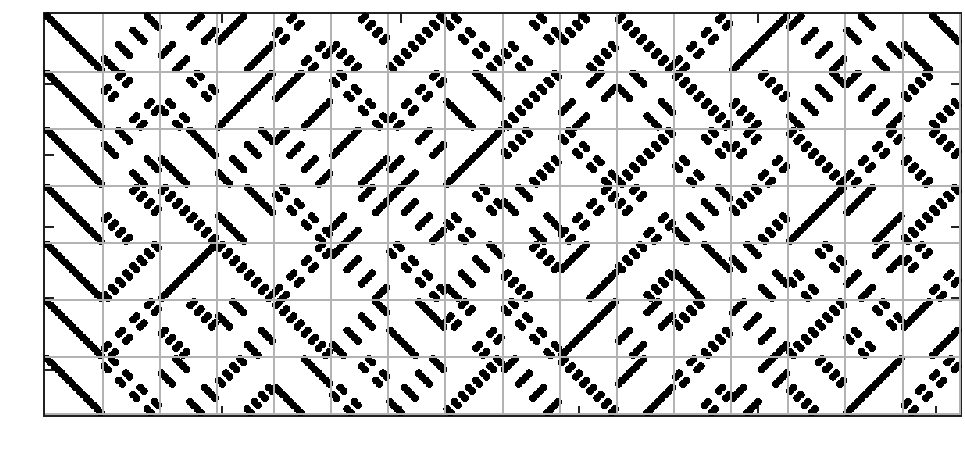
\includegraphics[width=\linewidth,height=0.52\textheight,keepaspectratio]{figures/Figure_1.pdf}
    \end{column}
  \end{columns}
  \pause
  \vspace{0.5cm}
  \begin{itemize}
    \item The lifted PCM $\bH$ contains a $4$-cycle from the blocks $\bD^{\psi(p_{i_1,j_1})}$, $\bD^{\psi{(p_{i_1,j_2})}}$, $\bD^{\psi{(p_{i_2,j_2}})}$, and $\bD^{\psi{(p_{i_2,j_1})}}$ iff~\citereference{BBS25}
    \[p_{i_1,j_1} + p_{i_2,j_1} = p_{i_2,j_2} + p_{i_1,j_2}, \quad i_1\neq i_2, j_1\neq j_2\]
  \end{itemize}
  \vspace{0.4cm}
  \addreferences
    {BBS25}{A.~Baldelli, M.~Battaglioni, and P.~Santini, ``Quantum {CSS} {LDPC} codes with quasi-dyadic structure,'' in \emph{Proc. ISTC}, 2025.}
  \endreferences
\end{frame}

\begin{frame}[c]{Dyadic CAMEL Codes: Girth-6 Components}
  \begin{columns}[T,onlytextwidth]
    \begin{column}{\textwidth}
      \begin{itemize}
        \item We now first construct QD component matrices \(\bH\)
        of girth $6$
      \end{itemize}
        \begin{center}
          \begin{minipage}{0.89\textwidth}
            \begin{theobox}{\textbf{Girth $6$ condition for QD matrices}}{
              Let $\bP\in\Fq^{w\times 2^\ell}$ be generated by
              \[
                p_{u,j}=a_u\lambda_j+b_u
              \]
              where the multipliers $a_u\in\Fq\backslash\{0\}$ are all distinct and $\lambda_j = \psi^{-1} (j)$. Then, the QD matrix lifted from $\bP$ has girth at least $6$.}
            \end{theobox}
          \end{minipage}
        \end{center}
\vspace{-1em}
        \begin{itemize}
          \item Proof idea
          \begin{itemize}
            \item Property of DPMs
            \[ \bD^{\psi(i)}\bD^{\psi(j)}=\bD^{\psi(i + j)}\]
            \item If all multipliers $a_u$ are distinct, then the product of two DPMs $\bD^{\psi(p_{u,j})}\bD^{\psi(p_{v,j})}=\bD^{\psi(p_{u,j} + p_{v,j})}$ depends on
            \[
              p_{u,j}+p_{v,j}
              =(a_u+a_v)\lambda_j+(b_u+b_v),
            \]
            which is a permutation of $\Fq$.

          \end{itemize}

        \end{itemize}



%      \begin{itemize}
%        \item Use the same affine-row design for both components:
%        \[
%          p^{(M)}_{u,j}
%          =a^{(M)}_u\lambda_j+b^{(M)}_u,
%          \qquad M\in\{1,2\}.
%        \]
%
%        \item Distinct $a_u,a_v$ imply $a_u+a_v\neq 0$.
%        \item Thus every row pair sees each XOR difference at most once.
%        \item A $4$-cycle would require a repeated row-pair difference.
%      \end{itemize}
    \end{column}
  \end{columns}
\end{frame}

\begin{frame}[c]{Dyadic CAMEL Codes: CSS Construction}


  \begin{enumerate}
    \item Start from $\bP\in\Fq^{w\times 2^\ell}$ generated by \(p_{u,j}=a_u\lambda_j+b_u\)
    \item Lift $\bP$ to QD PCM $\bH \in \mathbb{F}_2^{w 2^{\ell} \times 2^{2\ell}}$
    \item Perform partitioning
    \[\bH =: \begin{pmatrix} \bH_1 \\ \bH_2
    \end{pmatrix}\]

    \item Both $ \bH_1 $ and $ \bH_2 $ have girth at least 6 and
    \[ \bH_1\bH_2^\top=\bone .\]

    \item Append the all-one column to obtain the CSS matrices $\bH_X,\bH_Z$
  \end{enumerate}
\end{frame}


\begin{frame}[c]{Constructed Codes}
  \begin{columns}[T,onlytextwidth]
    \begin{column}{0.95\textwidth}
      \begin{itemize}
        \item Let $w=3$, $\ell=3$, and work over
        \(
          \mathbb{F}_8=\mathbb{F}_2[x]/\langle x^3+x+1\rangle.
        \)
        Construct the exponent matrix
      \[
      \bP=
      \begin{pmatrix}
      1 & \alpha^3 & \alpha^6 & \alpha^5 & \alpha & 0 & \alpha^4 & \alpha^2 \\
      \alpha^2 & 0 & \alpha^5 & \alpha^3 & \alpha & \alpha^4 & 1 & \alpha^6 \\
      \alpha^4 & 0 & 1 & \alpha^5 & \alpha^3 & \alpha^6 & \alpha^2 & \alpha\\
      \hline
      \alpha & \alpha^3 & 0 & 1 & \alpha^4 & \alpha^5 & \alpha^2 & \alpha^6 \\
      \alpha^6 & \alpha^4 & \alpha^3 & 0 & \alpha & 1 & \alpha^2 & \alpha^5 \\
      1 & \alpha^2 & 0 & \alpha^6 & \alpha^3 & \alpha^4 & \alpha & \alpha^5
      \end{pmatrix}
      \]

    \item Use $\ell\in\{4,5\}$, i.e., fields $\mathbb{F}_{16}$ and $\mathbb{F}_{32}$, and construct the codes

        \vspace{0.2cm}
      \centering
      \small
      \begin{tabular}{ccccccc}
        \toprule
        Code & $n$ & $k$ & $R_Q$ & $\ell$ & $d_{\mathsf{c}}'$ & $d_{\mathsf{v}}'$\\
        \midrule
        D1 & 257 & 121 & 0.47 & 4 & 16 & 7\\
        D2 & 1025 & 583 & 0.57 & 5 & 32 & 15\\
        \bottomrule
      \end{tabular}
      \end{itemize}
    \end{column}
  \end{columns}
\end{frame}

%\begin{frame}[c]{Constructed Codes}
%  \begin{columns}[T,onlytextwidth]
%    \begin{column}{0.48\textwidth}
%      \begin{itemize}
%        \item Use $\ell\in\{4,5\}$, i.e., fields $\mathbb{F}_{16}$ and $\mathbb{F}_{32}$.
%        \item Split the nonzero field elements into disjoint multiplier sets:
%        \[
%          |\mathcal{A}_X|=|\mathcal{A}_Z|=2^{\ell-1}-1 .
%        \]
%        \item Set $b=0$, lift by DPMs, then append the all-one column:
%        \[
%          n=2^{2\ell}+1 .
%        \]
%        \item Use overcomplete $\bH_X,\bH_Z$ for improved BP decoding.
%      \end{itemize}
%    \end{column}
%    \begin{column}{0.47\textwidth}
%      \centering
%      \small
%      \begin{tabular}{ccccccc}
%      \toprule
%      Code & $n$ & $k$ & $R_Q$ & $\ell$ & $d_{\mathsf{c}}'$ & $d_{\mathsf{v}}'$\\
%      \midrule
%      D1 & 257 & 121 & 0.47 & 4 & 16 & 7\\
%      D2 & 1025 & 583 & 0.57 & 5 & 32 & 15\\
%      \bottomrule
%      \end{tabular}
%
%      \vspace{0.45cm}
%      \begin{beamerboxesrounded}[upper=color_upper,lower=color_lower,width=0.93\textwidth]{Rate note}
%        \footnotesize The achieved rates are larger than the simple lower bound because the component check matrices are overcomplete.
%      \end{beamerboxesrounded}
%    \end{column}
%  \end{columns}
%\end{frame}

\begin{frame}[c]{Simulation Setup}
  \begin{itemize}
    \item \schlagwort{Depolarizing channel} with error probability $p$
    \item \schlagwort{Sum-product BP} using a \schlagwort{flooding schedule} with 15 iterations
    \item Each point simulated until 100 logical errors are detected
    \item Compare the following decoders
  \end{itemize}

  \begin{columns}[t,onlytextwidth]
    \begin{column}{0.05\textwidth}
      \textcolor{white}{xxxx}
    \end{column}
    \begin{column}{0.3\textwidth}
      \begin{minipage}[c][2.9cm][c]{\linewidth}
          \vspace{-1em}
        \begin{itemize}
          \item<2-> Plain \BPfour{} decoding
          \item<3-> CAMEL decoding
          \item<4-> Genie-aided decoding
        \end{itemize}
      \end{minipage}

    \end{column}
    \begin{column}{0.4\textwidth}
      \begin{minipage}[c][2.9cm][c]{\linewidth}
      \centering
      \visible<2->{\resizebox{\linewidth}{!}{%		\tikzset{line/.style={-latex},
%      branch highlight/.style={draw=KITpalegreen!45,line width=7pt,line cap=round,line join=round}}
%		\begin{tikzpicture}
%    \node[draw=none] at (0,3.2) {\footnotesize$\bm{z}$};
%    \node[draw,circle,fill,inner sep=1pt] at (0.3,3)(s) {};
%    \node[draw,circle,fill,inner sep=1pt] at (0.3,3.3) (s1){};
%    \node[draw,circle,fill,inner sep=1pt] at (0.3,2.7) (s2) {};
%
%    \draw[very thick] (-0.2,3) -- (s);
%
%    \only<4->{\draw[branch highlight] (s1) |- (2,3.9);}
%    \alt<4->{\draw[very thick,fill=KITpalegreen!30] (2,3.7) rectangle ++(1,0.4);}{\draw[very thick] (2,3.7) rectangle ++(1,0.4);}
%    \node[draw=none] at (1,4.1) {\footnotesize $\mathsf{v}_n=0$};
%    \node[draw=none] at (2.5,3.9)(BP1) {\footnotesize BP};
%    \draw[line, very thick] (s1) |- (2,3.9);
%
%    \draw[very thick] (2,3.1) rectangle ++(1,0.4);
%    \node[draw=none] at (1,3.5) {\footnotesize $\mathsf{v}_n=1$};
%    \node[draw=none] at (2.5,3.3)(BP2) {\footnotesize BP};
%    \draw[line, very thick] (s) |- (2,3.3);
%
%    \draw[very thick] (2,2.5) rectangle ++(1,0.4);
%    \node[draw=none] at (1,2.9) {\footnotesize $\mathsf{v}_n=\omega$};
%    \node[draw=none] at (2.5,2.7)(BP3) {\footnotesize BP};
%    \draw[line, very thick] (s) |- (2,2.7);
%    \draw[very thick] (2,1.9) rectangle ++(1,0.4);
%    \node[draw=none] at (1,2.3) {\footnotesize $\mathsf{v}_n=\bar{\omega}$};
%    \node[draw=none] at (2.5,2.1)(BP4) {\footnotesize BP};
%    \draw[line,very thick] (s2) |- (2,2.1);
%
%    \node[draw,rectangle,text width=0.4cm, minimum height=1cm,align=center,very thick] at (4.5,3)(w) {\footnotesize ML};
%
%    \node[draw=none] at (3.5,4.1) {\footnotesize $\hat{\bm{e}}_0$};
%    \node[draw=none] at (3.5,3.5) {\footnotesize $\hat{\bm{e}}_1$};
%    \node[draw=none] at (3.5,2.9) {\footnotesize $\hat{\bm{e}}_2$};
%    \node[draw=none] at (3.5,2.3) {\footnotesize $\hat{\bm{e}}_3$};
%
%    \only<4->{\draw[branch highlight] (3,3.9) -| (w);}
%    \draw[line, very thick] (3,3.9) -| (w);
%    \draw[line, very thick] (3,3.3) -- (4.2,3.3);
%    \draw[line, very thick] (3,2.7) -- (4.2,2.7);
%    \draw[line, very thick] (3,2.1) -| (w);
%
%     \node[draw=none] at (5.5,3.2) {\footnotesize$\hat{\bm{e}}$};
%     \draw[line, very thick] (w) -- (6,3);
%     \end{tikzpicture}


\tikzset{
  line/.style={-{Latex}, very thick},
  active line/.style={-{Latex}, very thick, draw=KITpalegreen!70!black},
  bp/.style={very thick},
  bp active/.style={very thick, draw=KITpalegreen!70!black, fill=KITpalegreen!30}
}

\begin{tikzpicture}
    % Left input
    \visible<3->{
    \node[draw=none] at (0,3.2) {\footnotesize$\bm{z}$};
    \node[draw,circle,fill,inner sep=1pt] at (0.3,3)   (s)  {};

    \node[draw,circle,fill,inner sep=1pt] at (0.3,2.7) (s2) {};

    \draw[very thick] (-0.2,3) -- (s);
        \node[draw,circle,fill,inner sep=1pt] at (0.3,3.3) (s1) {};
    }



    % BP blocks
    \alt<4->{\draw[bp active] (2,3.7) rectangle ++(1,0.4);}
    {\draw[bp] (2,3.7) rectangle ++(1,0.4);}
    \visible<3->{
    \draw[bp] (2,3.1) rectangle ++(1,0.4);
    \draw[bp] (2,2.5) rectangle ++(1,0.4);
    \draw[bp] (2,1.9) rectangle ++(1,0.4);


    % Labels for branches
    \node[draw=none] at (1,4.1) {\footnotesize $\mathsf{v}_n=0$};
    \node[draw=none] at (1,3.5) {\footnotesize $\mathsf{v}_n=1$};
    \node[draw=none] at (1,2.9) {\footnotesize $\mathsf{v}_n=\omega$};
    \node[draw=none] at (1,2.3) {\footnotesize $\mathsf{v}_n=\bar{\omega}$};
    }
    \visible<3->{
    % BP text

    \node[draw=none] at (2.5,3.3) (BP2) {\footnotesize BP};
    \node[draw=none] at (2.5,2.7) (BP3) {\footnotesize BP};
    \node[draw=none] at (2.5,2.1) (BP4) {\footnotesize BP};
    }
    \node[draw=none] at (2.5,3.9) (BP1) {\footnotesize BP};
    \visible<2>{
    \draw[line]        (0.3,3.9) -- (2,3.9);
    \draw[line]        (3,3.9) -- (4.5,3.9);
    }
    % Connections from BP blocks to ML

    \visible<3->{

    % Connections from left to BP blocks
        \alt<4->{\draw[active line] (s1) |- (2,3.9);}
        {\draw[line]        (s1) |- (2,3.9);}

    \draw[line] (s)  |- (2,3.3);
    \draw[line] (s)  |- (2,2.7);
    \draw[line] (s2) |- (2,2.1);
    \alt<4->{\draw[active line] (3,3.9) -| (w);}
        {\draw[line]        (3,3.9) -| (w);}
    % ML block
    \node[
        draw,
        rectangle,
        text width=0.4cm,
        minimum height=1cm,
        align=center,
        very thick
    ] at (4.5,3) (w) {\footnotesize ML};

    % Labels between BP and ML
    \node[draw=none] at (3.5,4.1) {\footnotesize $\hat{\bm{e}}_0$};
    \node[draw=none] at (3.5,3.5) {\footnotesize $\hat{\bm{e}}_1$};
    \node[draw=none] at (3.5,2.9) {\footnotesize $\hat{\bm{e}}_2$};
    \node[draw=none] at (3.5,2.3) {\footnotesize $\hat{\bm{e}}_3$};


    \draw[line] (3,3.3) -- (4.2,3.3);
    \draw[line] (3,2.7) -- (4.2,2.7);
    \draw[line] (3,2.1) -| (w);

    % Output
    \node[draw=none] at (5.5,3.2) {\footnotesize$\hat{\bm{e}}$};
    \draw[line] (w) -- (6,3);
    }
\end{tikzpicture}}}
      \end{minipage}
    \end{column}

    \begin{column}{0.25\textwidth}
      \textcolor{white}{xxxx}
    \end{column}

  \end{columns}
\end{frame}

\begin{frame}[c]{Numerical Results: D1 Code}
  \begin{columns}[c,onlytextwidth]
    \begin{column}{0.5\textwidth}
      \centering
      \visible<2->{\resizebox{0.98\textwidth}{!}{\tikzset{
  alt/.code args={<#1>#2#3}{%
    \alt<#1>{\pgfkeysalso{#2}}{\pgfkeysalso{#3}}%
  },
  visible on/.style={alt={#1{}{opacity=0}}},
}
        \begin{tikzpicture}
		\pgfplotsset{grid style={dashed, gray}}
		\pgfplotsset{every tick label/.append style={font=\footnotesize}}
		
		\begin{axis}[%
		xshift=1.5cm,
		xmin=0.0005,
		xmax=0.1,
		ymode=log,
        xmode = log,
		ymin=9e-6,
		ymax=1,
		yminorticks=true,
		axis background/.style={fill=white, mark size=1.5pt},
		xmajorgrids,
		ymajorgrids,
		%yminorgrids,
		width=6.5cm,
        height=6cm,
		% xtick={2.5, 2.8,...,5.5},
		% ytick={0.1,0.01,0.001,1e-4,1e-5,1e-6,1e-7,1e-8, 1e-9,1e-10,1e-11,1e-12,1e-13,1e-14},
		xlabel={Depolarizing probability $p$},
		xlabel style={yshift=0.35em},
		ylabel={LER},
		label style={font=\small},
		legend cell align={left},
		legend style={anchor = north west,  at={(0,1)}, draw=none, fill opacity=0, text opacity = 1,legend columns=1,font=\footnotesize, row sep = 0pt}
		]

% Plain BP4: visible from overlay 2
\addplot[
  color=black,
  mark=triangle,
  dashed,
  mark options={solid},
  line width=0.5pt,
  visible on=<2->
]
table[row sep=crcr] {
  0.05 1e-19\\
};
\addlegendentry{\visible<2->{Plain BP4}}

% CAMEL decoding: visible from overlay 3
\addplot[
  color=black,
  mark=o,
  mark options={solid},
  line width=0.5pt,
  visible on=<3->
]
table[row sep=crcr] {
  0.05 1e-19\\
};
\addlegendentry{\visible<3->{CAMEL decoding}}



% Genie-aided BP4: visible from overlay 4
\addplot[
  color=black,
  mark=square,
  dotted,
  mark options={solid},
  line width=0.5pt,
  visible on=<4->
]
table[row sep=crcr] {
  0.05 1e-19\\
};

\addlegendentry{\visible<4->{Genie-aided BP4}}

% D1 code: visible from overlay 2
\addplot[
  color=blue,
  line width=0.5pt,
  visible on=<2->
]
table[row sep=crcr] {
  0.05 1e-19\\
};
\addlegendentry{\visible<2->{New: D1 code}}

% C1 code: visible from overlay 2
\addplot[
  color=KITpalegreen,
  line width=0.5pt,
  visible on=<2->
]
table[row sep=crcr] {
  0.05 1e-19\\
};
\addlegendentry{\visible<2->{C1 code}}

% H1 code: visible from overlay 2
\addplot[
  color=black!50!red,
  dashed,
  line width=0.5pt,
  mark=star,
  mark options={solid},
  mark size=2pt,
  visible on=<2->
]
table[row sep=crcr] {
  0.05 1e-19\\
};
\addlegendentry{\visible<2->{H1 code}}
% %D4 code ========================================================
% % 65_27 code --> removed from paper
% \addplot[
%     mark=o,
%     color=green!50!blue,
%     mark=triangle,mark options={solid},dashed,
%     line width = 0.5pt
% ]
% table[row sep=crcr] {
% % collect 1000 frame errors or 60000000 decoded error patterns
% % depolarizing prob. list to be simulated: 0.1, 0.05, 0.025, 0.0125, 0.00625, 0.003125, 0.0015625, 0.00078125, 0.000390625, 0.000195313, 
% % Decoding option: Flooding BP========================
% % [[65,27]], 48 checks, 15 iter, ep0=0.1
% % FE 1055, total dec. 1387\\
% 0.1 0.760634\\
% % FE 1032, total dec. 3879\\
% 0.05 0.266048\\
% % FE 1014, total dec. 12929\\
% 0.025 0.0784283\\
% % FE 1013, total dec. 46246\\
% 0.0125 0.0219046\\
% % FE 1003, total dec. 157474\\
% 0.00625 0.00636931\\
% % FE 1002, total dec. 664080\\
% 0.003125 0.00150885\\
% % FE 1001, total dec. 2.46016e+06\\
% 0.0015625 0.000406884\\
% % FE 1001, total dec. 9.74861e+06\\
% 0.00078125 0.000102681\\
% % FE 244, total dec. 1e+07\\
% % FE 495, total dec. 2e+07\\
% % FE 769, total dec. 3e+07\\
% % FE 1001, total dec. 3.95889e+07\\
% 0.000390625 2.52849e-05\\
% % FE 59, total dec. 1e+07\\
% % FE 123, total dec. 2e+07\\
% % FE 173, total dec. 3e+07\\
% % FE 219, total dec. 4e+07\\
% % FE 289, total dec. 5e+07\\
% % FE 343, total dec. 6e+07\\
% % FE 343, total dec. 6.00001e+07\\
% 0.000195313 5.71666e-06\\
% };


% \addplot[
%     mark=o,
%     color=green!50!blue,
%     mark=o,mark options={solid},
%     line width = 0.5pt
% ]
% table[row sep=crcr] {
% % collect 1000 frame errors or 60000000 decoded error patterns
% % depolarizing prob. list to be simulated: 0.1, 0.05, 0.025, 0.0125, 0.00625, 0.003125, 0.0015625, 0.00078125, 0.000390625, 0.000195313, 
% % Decoding option: CAMEL
% % [[65,27]], 48 checks, 15 iter, ep0=0.1
% % FE 1044, total dec. 1444\\
% 0.1 0.722992\\
% % FE 1019, total dec. 4003\\
% 0.05 0.254559\\
% % FE 1005, total dec. 13782\\
% 0.025 0.0729212\\
% % FE 1004, total dec. 49476\\
% 0.0125 0.0202927\\
% % FE 1002, total dec. 174768\\
% 0.00625 0.00573332\\
% % FE 1001, total dec. 675492\\
% 0.003125 0.00148188\\
% % FE 1003, total dec. 2.82248e+06\\
% 0.0015625 0.000355361\\
% % FE 924, total dec. 1e+07\\
% % FE 1001, total dec. 1.08338e+07\\
% 0.00078125 9.23959e-05\\
% % FE 1001, total dec. 4.35146e+07\\
% 0.000390625 2.30038e-05\\
% % FE 349, total dec. 6.00001e+07\\
% 0.000195313 5.81666e-06\\
% };
% %D4 code ========================================================

%D1 code ========================================================
\only<3->{%
\addplot[
    mark=o,
color=blue,
    line width = 0.5pt
]
table[row sep=crcr] {
% collect 100 frame errors or 60000000 decoded error patterns
% depolarizing prob. list to be simulated: 0.05, 0.025, 0.0125, 0.00625, 0.003125, 0.0015625, 0.00078125, 0.000390625, 0.000195313, 
% $\llbracket 257,121 \rrbracket$, 224 checks, 15 iter, ep0=0.1
% FE 487, total dec. 501\\
0.1 0.972056\\
% FE 473, total dec. 503\\
0.09 0.940358\\
% FE 459, total dec. 573\\
0.08 0.801047\\
% FE 444, total dec. 684\\
0.07 0.649123\\
% FE 379, total dec. 994\\
0.06 0.381288\\
% FE 344, total dec. 1968\\
0.05 0.174797\\
% FE 313, total dec. 6205\\
0.04 0.0504432\\
% FE 304, total dec. 51148\\
0.03 0.00594354\\
% FE 301, total dec. 985734\\
0.02 0.000305356\\
% FE 301, total dec. 1.97093e+06\\
0.018 0.00015272\\
% FE 301, total dec. 5.6135e+06\\
0.016 5.36207e-05\\
% FE 301, total dec. 1.26876e+07\\
0.014 2.37239e-05\\
% FE 301, total dec. 3.29437e+07\\
0.012 9.13681e-06\\
};
}%


\only<4->{%
\addplot[
    mark=square,
color=blue, dotted,
    mark=square,mark options={solid},
    line width = 0.5pt
]
table[row sep=crcr] {
% collect 300 frame errors or 60000000 decoded error patterns
% depolarizing prob. list to be simulated: 0.1, 0.05, 0.025, 0.0125, 
% Decoding option: Genie-aided BP
% [[257,121]], 224 checks, 15 iter, ep0=0.1
% FE 364, total dec. 375\\
0.1 0.970667\\
% FE 344, total dec. 613\\
0.0666667 0.561175\\
% FE 315, total dec. 3418\\
0.0444444 0.0921592\\
% FE 301, total dec. 50861\\
0.0296296 0.00591809\\
% FE 301, total dec. 1.19484e+06\\
0.0197531 0.000251917\\
% FE 301, total dec. 2.01864e+07\\
0.0131687 1.4911e-05\\
};
}%

\only<2->{%
\addplot[
    mark=triangle,
 color=blue, dashed,
    mark options={solid},
    line width = 0.5pt
]
table[row sep=crcr] {
% collect 300 frame errors or 60000000 decoded error patterns
% depolarizing prob. list to be simulated: 0.1, 0.0666667, 0.0444444, 0.0296296, 0.0197531, 0.0131687, 0.00877915, 0.00585277, 0.00390184, 0.00260123, 0.00173415, 0.0011561, 
% Decoding option: Flooding BP
% [[257,121]], 224 checks, 15 iter, ep0=0.1
% FE 425, total dec. 433\\
0.1 0.981524\\
% FE 392, total dec. 714\\
0.0666667 0.54902\\
% FE 330, total dec. 3097\\
0.0444444 0.106555\\
% FE 311, total dec. 15489\\
0.0296296 0.0200788\\
% FE 308, total dec. 29282\\
0.0197531 0.0105184\\
% FE 306, total dec. 39631\\
0.0131687 0.00772123\\
% FE 304, total dec. 63846\\
0.00877915 0.00476146\\
% FE 303, total dec. 105845\\
0.00585277 0.00286268\\
% FE 301, total dec. 217088\\
0.00390184 0.00138653\\
% FE 302, total dec. 442057\\
0.00260123 0.00068317\\
% FE 301, total dec. 758098\\
0.00173415 0.000397046\\
% FE 301, total dec. 1.87322e+06\\
0.0011561 0.000160686\\
};
}%


%D1 code ========================================================



%C1 code ========================================================
\only<3->{%
\addplot[
    mark=o,
color=KITpalegreen,
    line width = 0.5pt
]
table[row sep=crcr] {
% check symplectic ok
% collect 300 frame errors or 100000000 decoded error patterns
% depolarizing prob. list to be simulated: 0.12, 0.11, 0.1, 0.09, 0.08, 0.07, 0.06, 0.05, 0.04, 0.03, 0.02, 0.018, 
% Decoding option: CAMEL
% [[290,128]], 170 checks, 15 iter, ep0=0.1
% FE 320, total dec. 320\\
0.12 1\\
% FE 320, total dec. 320\\
0.11 1\\
% FE 320, total dec. 320\\
0.1 1\\
% FE 319, total dec. 320\\
0.09 0.996875\\
% FE 320, total dec. 327\\
0.08 0.978593\\
% FE 319, total dec. 344\\
0.07 0.927326\\
% FE 317, total dec. 384\\
0.06 0.825521\\
% FE 314, total dec. 533\\
0.05 0.589118\\
% FE 307, total dec. 1066\\
0.04 0.287992\\
% FE 302, total dec. 4316\\
0.03 0.0699722\\
% FE 301, total dec. 59801\\
0.02 0.00503336\\
% FE 301, total dec. 113787\\
0.018 0.00264529\\
% collect 300 frame errors or 100000000 decoded error patterns
% depolarizing prob. list to be simulated: 0.016, 0.014, 0.012, 
% Decoding option: CAMEL
% [[290,128]], 170 checks, 15 iter, ep0=0.1
% FE 301, total dec. 246331\\
0.016 0.00122193\\
% FE 302, total dec. 666356\\
0.014 0.000453211\\
};
}%


\only<4->{%
\addplot[
    mark=square,
color=KITpalegreen,
    mark=square,mark options={solid},
    line width = 0.5pt
]
table[row sep=crcr] {
% collect 300 frame errors or 100000000 decoded error patterns
% depolarizing prob. list to be simulated: 0.12, 0.11, 0.1, 0.09, 0.08, 0.07, 0.06, 0.05, 0.04, 0.03, 0.02, 0.018, 0.016, 0.014, 0.012, 
% Decoding option: Genie-aided BP
% [[290,128]], 170 checks, 15 iter, ep0=0.1
% FE 320, total dec. 320\\
0.12 1\\
% FE 320, total dec. 320\\
0.11 1\\
% FE 320, total dec. 320\\
0.1 1\\
% FE 319, total dec. 325\\
0.09 0.981538\\
% FE 320, total dec. 325\\
0.08 0.984615\\
% FE 320, total dec. 342\\
0.07 0.935673\\
% FE 319, total dec. 387\\
0.06 0.824289\\
% FE 315, total dec. 574\\
0.05 0.54878\\
% FE 311, total dec. 1134\\
0.04 0.27425\\
% FE 305, total dec. 4192\\
0.03 0.0727576\\
% FE 301, total dec. 58957\\
0.02 0.00510542\\
% FE 301, total dec. 121538\\
0.018 0.00247659\\
% FE 301, total dec. 251262\\
0.016 0.00119795\\
% FE 301, total dec. 625529\\
0.014 0.000481193\\
% FE 301, total dec. 1.71533e+06\\
0.012 0.000175477\\
};
}%

\only<2->{%
\addplot[
    mark=triangle,
 color=KITpalegreen, dashed,
    mark options={solid},
    line width = 0.5pt
]
table[row sep=crcr] {
% collect 300 frame errors or 100000000 decoded error patterns
% depolarizing prob. list to be simulated: 0.1, 0.09, 0.08, 0.07, 0.06, 0.05, 0.04, 0.03, 0.02, 0.01, 0.009, 0.008, 0.007, 0.006, 0.005, 0.004, 0.003, 0.002, 0.001, 0.001, 
% Decoding option: Flooding BP
% [[290,128]], 170 checks, 15 iter, ep0=0.1
% FE 320, total dec. 320\\
0.1 1\\
% FE 319, total dec. 321\\
0.09 0.993769\\
% FE 320, total dec. 325\\
0.08 0.984615\\
% FE 320, total dec. 343\\
0.07 0.932945\\
% FE 319, total dec. 388\\
0.06 0.822165\\
% FE 317, total dec. 522\\
0.05 0.60728\\
% FE 306, total dec. 1139\\
0.04 0.268657\\
% FE 303, total dec. 4421\\
0.03 0.0685365\\
% FE 301, total dec. 39311\\
0.02 0.00765689\\
% FE 301, total dec. 110948\\
0.01 0.00271298\\
% FE 301, total dec. 112209\\
0.009 0.00268249\\
% FE 301, total dec. 125543\\
0.008 0.00239758\\
% FE 301, total dec. 149936\\
0.007 0.00200752\\
% FE 301, total dec. 193880\\
0.006 0.00155251\\
% FE 301, total dec. 232554\\
0.005 0.00129432\\
% FE 301, total dec. 314905\\
0.004 0.000955844\\
% FE 301, total dec. 565463\\
0.003 0.000532307\\
% FE 301, total dec. 999186\\
0.002 0.000301245\\
% FE 301, total dec. 3.62873e+06\\
0.001 8.2949e-05\\
};
}%
%C1 code ========================================================



\only<2->{%
\addplot [color=black!50!red, dashed, line width=0.5pt,mark=star, mark options={solid}, mark size = 2pt]table[row sep=crcr]{
    0.08995451958872763 0.8074878458635921\\
0.07910314675722364 0.6107653946066945\\
0.06956079422694146 0.4151195836467042\\
0.06140126800498785 0.26462050618904925\\
0.049872983923963235 0.1197102765411727\\
0.03990113244336744 0.05531797752399404\\
0.029935772947204904 0.02295631924236914\\
0.01989988536895992 0.006615389893015433\\
0.009924666630948488 0.0008435452308265797\\
};
}%
% \addlegendentry{H1 code};



\end{axis}
\end{tikzpicture}
}}
    \end{column}
    \begin{column}{0.5\textwidth}
      \begin{tabular}{lccl}
        \toprule
        Code & $n$ & $k$ & Decoder\\
        \midrule
        D1 & 257 & 121 & CAMEL\\
        C1~\citereference{CAMEL} & 290 & 128 & CAMEL\\
        \visible<4>{H1~\citereference{TZ13}} & \visible<4>{400} & \visible<4>{16} & \visible<4>{BP+OSD~\citereference{RWBC20}}\\
        \bottomrule
      \end{tabular}

      \visible<2->{%
      \vspace{0.5cm}
      \begin{itemize}
        \item Plain \BPfour{} shows an error floor
        \visible<3->{%
        \item CAMEL suppresses the floor \visible<4->{and matches genie-aided \BPfour}
        }
        \visible<4->{%
        \item D1 with CAMEL outperforms C1 and H1 despite higher rate and shorter block length
        }
      \end{itemize}
      }
    \end{column}
  \end{columns}
  \vspace{0.4cm}

  \noindent\hspace*{-0.35cm}%
  {\scriptsize
  \renewcommand{\arraystretch}{1}
    \begin{tabular}{lp{0.93\textwidth}}
      \textcolor{kit-green100}{[TZ13]} &
      \textcolor{kit-green100}{J.-P.~Tillich and G.~Z\'emor, ``Quantum {LDPC} codes with positive rate and minimum distance proportional to $\sqrt{n}$,'' \emph{TIT}, 2013.}\\
      \visible<4>{\textcolor{kit-green100}{[RWBC20]} &
      \textcolor{kit-green100}{J.~Roffe, D.~R. White, S.~Burton, and E.~Campbell, ``Decoding across the quantum low-density parity-check code landscape,'' \emph{Physical Review Research}, 2020.}}
    \end{tabular}
  }

%  \addreferences
%%  {CAMEL}{S.~Miao, J.~Mandelbaum, H.~J\"akel, and L.~Schmalen, ``A joint code and belief propagation decoder design for quantum {LDPC} codes,'' in \emph{Proc. IEEE Int. Symp. Inform. Theory (ISIT)}, Athens, Greece, Jul.~2024.}
%  {TZ13}{J.-P.~Tillich and G.~Z\'emor, ``Quantum {LDPC} codes with positive rate and minimum distance proportional to the square root of the blocklength,'' \emph{IEEE Trans. Inf. Theory}, 2013.}
%  {RWBC20}{J.~Roffe, D.~R. White, S.~Burton, and E.~Campbell, ``Decoding across the quantum low-density parity-check code landscape,'' \emph{Physical Review Research}, 2020.}
%  \endreferences
\end{frame}


\begin{frame}[c]{Conclusion}
  \begin{columns}[T,onlytextwidth]
    \begin{column}{0.85\textwidth}
      \small
      \begin{itemize}
        \item \schlagwort{CAMEL} framework provides a way to construct \schlagwort{BP-suitable QLDPC codes}
        \item \schlagwort{Quasi-dyadic codes} are an interesting code family with \schlagwort{rich algebraic structure}
        \item Constructed quasi-dyadic codes provide \schlagwort{competitive performance} at high coding rates
      \end{itemize}
    \end{column}
    \begin{column}{0.1\textwidth}
      \centering
      \vspace{0.1cm}
      
\includegraphics[width=\linewidth]{figures/camel.pdf}
    \end{column}
  \end{columns}

  \vspace{2cm}
  \begin{center}
    {\Huge\bfseries\textcolor{kit-green100}{Questions?}}
  \end{center}
  \vspace{-0.02cm}

  \begin{columns}[c,onlytextwidth]
    \begin{column}{0.17\textwidth}
      \centering
      \includegraphics[width=0.78\linewidth]{\templates/logos/LOGO_ERC-FLAG_EU.pdf}
    \end{column}
    \begin{column}{0.15\textwidth}
      \centering
      \includegraphics[width=0.62\linewidth]{\templates/logos/BMFTR_en_crop.pdf}
    \end{column}
    \begin{column}{0.64\textwidth}
      \scriptsize Funding: European Research Council (ERC), European Union's Horizon 2020 research and innovation programme, grant agreement No. 101001899; German Federal Ministry of Research, Technology and Space (BMFTR), Open6GHub+, grant agreement 16KIS2405.
    \end{column}
  \end{columns}
\end{frame}

\appendix




\begin{frame}[c,noframenumbering]{Backup: DPM Product Example}
  \begingroup
  \setlength{\arraycolsep}{1.25pt}
  \renewcommand{\arraystretch}{0.76}


  In $\mathbb{F}_8=\Ftwo[\alpha]/\langle\alpha^3+\alpha+1\rangle$ with basis $\{1,\alpha,\alpha^2\}$:
  \[
    \begin{aligned}
      a&=\alpha+\alpha^2, & \psi(a)&=6, & \varphi(a)&=\begin{pmatrix}1&1&0\end{pmatrix}\\
      b&=\alpha^2, & \psi(b)&=4, & \varphi(b)&=\begin{pmatrix}1&0&0\end{pmatrix}\\
      a+b&=\alpha, & \psi(a+b)&=2, & \varphi(a+b)&=\begin{pmatrix}0&1&0\end{pmatrix}
    \end{aligned}
  \]
  \vspace{-0.28cm}
  \[
    6\oplus4=2,
    \qquad
    \bD^{(6)}\bD^{(4)}=\bD^{(2)}
  \]
  \vspace{-0.22cm}

  \begin{columns}[T,onlytextwidth]
    \begin{column}{0.48\textwidth}
      \centering
      {$\bD^{(6)}\bD^{(4)}$}
      \vspace{-0.18cm}

      {
      \[
        \DtwoExampleMatrix
      \]
      }
    \end{column}
    \begin{column}{0.48\textwidth}
      \centering
      { $\bD^{(2)}$}
      \vspace{-0.18cm}

      {
      \[
        \DtwoExampleMatrix
      \]
      }
    \end{column}
  \end{columns}
  \endgroup
\end{frame}

\appendix

\begin{frame}[c]{Numerical Results: D2 Code}
    \begin{columns}[T,onlytextwidth]
        \begin{column}{0.5\textwidth}
            \centering
            \resizebox{0.98\textwidth}{!}{		\begin{tikzpicture}
		\pgfplotsset{grid style={dashed, gray}}
		\pgfplotsset{every tick label/.append style={font=\footnotesize}}
		
		\begin{axis}[%
		xshift=1.5cm,
		xmin=0.0005,
		xmax=0.1,
		ymode=log,
            xmode = log,
		ymin=9e-6,
		ymax=1,
		yminorticks=true,
		axis background/.style={fill=white, mark size=1.5pt},
		xmajorgrids,
		ymajorgrids,
		%yminorgrids,
		width=6.5cm,
        height=6cm,
		% xtick={2.5, 2.8,...,5.5},
		% ytick={0.1,0.01,0.001,1e-4,1e-5,1e-6,1e-7,1e-8, 1e-9,1e-10,1e-11,1e-12,1e-13,1e-14},
		xlabel={Depolarizing probability $p$},
		xlabel style={yshift=0.35em},
		ylabel={LER},
		label style={font=\small},
		legend cell align={left},
		legend style={anchor = north west,  at={(0,1)}, draw=none, fill opacity=0, text opacity = 1,legend columns=1,font=\footnotesize, row sep = 0pt}
		]

\addplot[color=black, mark=o, mark options={solid}, line width=0.5pt]
table[row sep=crcr] {
0.05 1e-19\\
};

\addplot[color=black, mark=triangle, dashed, mark options={solid}, line width=0.5pt]
table[row sep=crcr] {
0.05 1e-19\\
};

\addplot[color=black, mark=square, dotted, mark options={solid}, line width=0.5pt]
table[row sep=crcr] {
0.05 1e-19\\
};

\addplot[color=orange, line width=0.5pt]
table[row sep=crcr] {
0.05 1e-19\\
};

\addplot[color=KITorange, line width=0.5pt]
table[row sep=crcr] {
0.05 1e-19\\
};

\addplot[color=KITred, line width=1pt]
table[row sep=crcr] {
0.05 1e-19\\
};

\addplot[color=magenta, dashed, mark=star, mark options={solid}, line width=0.5pt]
table[row sep=crcr] {
0.05 1e-19\\
};


% \addlegendentry{Q4 code};
% \addlegendentry{D1 code};
\addlegendentry{CAMEL decoding};
\addlegendentry{Plain BP4};
\addlegendentry{Genie-aided BP4};
\addlegendentry{New: D2 code};
% \addlegendentry{C1 code};
\addlegendentry{C2 code};
\addlegendentry{E5 code}
\addlegendentry{B1 code}


% %D4 code ========================================================
% % 65_27 code --> removed from paper
% \addplot[
%     mark=o,
%     color=green!50!blue,
%     mark=triangle,mark options={solid},dashed,
%     line width = 0.5pt
% ]
% table[row sep=crcr] {
% % collect 1000 frame errors or 60000000 decoded error patterns
% % depolarizing prob. list to be simulated: 0.1, 0.05, 0.025, 0.0125, 0.00625, 0.003125, 0.0015625, 0.00078125, 0.000390625, 0.000195313, 
% % Decoding option: Flooding BP========================
% % [[65,27]], 48 checks, 15 iter, ep0=0.1
% % FE 1055, total dec. 1387\\
% 0.1 0.760634\\
% % FE 1032, total dec. 3879\\
% 0.05 0.266048\\
% % FE 1014, total dec. 12929\\
% 0.025 0.0784283\\
% % FE 1013, total dec. 46246\\
% 0.0125 0.0219046\\
% % FE 1003, total dec. 157474\\
% 0.00625 0.00636931\\
% % FE 1002, total dec. 664080\\
% 0.003125 0.00150885\\
% % FE 1001, total dec. 2.46016e+06\\
% 0.0015625 0.000406884\\
% % FE 1001, total dec. 9.74861e+06\\
% 0.00078125 0.000102681\\
% % FE 244, total dec. 1e+07\\
% % FE 495, total dec. 2e+07\\
% % FE 769, total dec. 3e+07\\
% % FE 1001, total dec. 3.95889e+07\\
% 0.000390625 2.52849e-05\\
% % FE 59, total dec. 1e+07\\
% % FE 123, total dec. 2e+07\\
% % FE 173, total dec. 3e+07\\
% % FE 219, total dec. 4e+07\\
% % FE 289, total dec. 5e+07\\
% % FE 343, total dec. 6e+07\\
% % FE 343, total dec. 6.00001e+07\\
% 0.000195313 5.71666e-06\\
% };


% \addplot[
%     mark=o,
%     color=green!50!blue,
%     mark=o,mark options={solid},
%     line width = 0.5pt
% ]
% table[row sep=crcr] {
% % collect 1000 frame errors or 60000000 decoded error patterns
% % depolarizing prob. list to be simulated: 0.1, 0.05, 0.025, 0.0125, 0.00625, 0.003125, 0.0015625, 0.00078125, 0.000390625, 0.000195313, 
% % Decoding option: CAMEL
% % [[65,27]], 48 checks, 15 iter, ep0=0.1
% % FE 1044, total dec. 1444\\
% 0.1 0.722992\\
% % FE 1019, total dec. 4003\\
% 0.05 0.254559\\
% % FE 1005, total dec. 13782\\
% 0.025 0.0729212\\
% % FE 1004, total dec. 49476\\
% 0.0125 0.0202927\\
% % FE 1002, total dec. 174768\\
% 0.00625 0.00573332\\
% % FE 1001, total dec. 675492\\
% 0.003125 0.00148188\\
% % FE 1003, total dec. 2.82248e+06\\
% 0.0015625 0.000355361\\
% % FE 924, total dec. 1e+07\\
% % FE 1001, total dec. 1.08338e+07\\
% 0.00078125 9.23959e-05\\
% % FE 1001, total dec. 4.35146e+07\\
% 0.000390625 2.30038e-05\\
% % FE 349, total dec. 6.00001e+07\\
% 0.000195313 5.81666e-06\\
% };
% %D4 code ========================================================

% %D1 code ========================================================
% \addplot[
%     mark=o,
% color=green!70!blue,
%     line width = 0.5pt
% ]
% table[row sep=crcr] {
% % collect 100 frame errors or 60000000 decoded error patterns
% % depolarizing prob. list to be simulated: 0.05, 0.025, 0.0125, 0.00625, 0.003125, 0.0015625, 0.00078125, 0.000390625, 0.000195313, 
% % $\llbracket 257,121 \rrbracket$, 224 checks, 15 iter, ep0=0.1
% % FE 487, total dec. 501\\
% 0.1 0.972056\\
% % FE 473, total dec. 503\\
% 0.09 0.940358\\
% % FE 459, total dec. 573\\
% 0.08 0.801047\\
% % FE 444, total dec. 684\\
% 0.07 0.649123\\
% % FE 379, total dec. 994\\
% 0.06 0.381288\\
% % FE 344, total dec. 1968\\
% 0.05 0.174797\\
% % FE 313, total dec. 6205\\
% 0.04 0.0504432\\
% % FE 304, total dec. 51148\\
% 0.03 0.00594354\\
% % FE 301, total dec. 985734\\
% 0.02 0.000305356\\
% % FE 301, total dec. 1.97093e+06\\
% 0.018 0.00015272\\
% % FE 301, total dec. 5.6135e+06\\
% 0.016 5.36207e-05\\
% % FE 301, total dec. 1.26876e+07\\
% 0.014 2.37239e-05\\
% % FE 301, total dec. 3.29437e+07\\
% 0.012 9.13681e-06\\
% };


% \addplot[
%     mark=square,
% color=green!70!blue, dotted,
%     mark=square,mark options={solid},
%     line width = 0.5pt
% ]
% table[row sep=crcr] {
% % collect 300 frame errors or 60000000 decoded error patterns
% % depolarizing prob. list to be simulated: 0.1, 0.05, 0.025, 0.0125, 
% % Decoding option: Genie-aided BP
% % [[257,121]], 224 checks, 15 iter, ep0=0.1
% % FE 364, total dec. 375\\
% 0.1 0.970667\\
% % FE 344, total dec. 613\\
% 0.0666667 0.561175\\
% % FE 315, total dec. 3418\\
% 0.0444444 0.0921592\\
% % FE 301, total dec. 50861\\
% 0.0296296 0.00591809\\
% % FE 301, total dec. 1.19484e+06\\
% 0.0197531 0.000251917\\
% % FE 301, total dec. 2.01864e+07\\
% 0.0131687 1.4911e-05\\
% };

% \addplot[
%     mark=triangle,
%  color=green!70!blue, dashed,
%     mark options={solid},
%     line width = 0.5pt
% ]
% table[row sep=crcr] {
% % collect 300 frame errors or 60000000 decoded error patterns
% % depolarizing prob. list to be simulated: 0.1, 0.0666667, 0.0444444, 0.0296296, 0.0197531, 0.0131687, 0.00877915, 0.00585277, 0.00390184, 0.00260123, 0.00173415, 0.0011561, 
% % Decoding option: Flooding BP
% % [[257,121]], 224 checks, 15 iter, ep0=0.1
% % FE 425, total dec. 433\\
% 0.1 0.981524\\
% % FE 392, total dec. 714\\
% 0.0666667 0.54902\\
% % FE 330, total dec. 3097\\
% 0.0444444 0.106555\\
% % FE 311, total dec. 15489\\
% 0.0296296 0.0200788\\
% % FE 308, total dec. 29282\\
% 0.0197531 0.0105184\\
% % FE 306, total dec. 39631\\
% 0.0131687 0.00772123\\
% % FE 304, total dec. 63846\\
% 0.00877915 0.00476146\\
% % FE 303, total dec. 105845\\
% 0.00585277 0.00286268\\
% % FE 301, total dec. 217088\\
% 0.00390184 0.00138653\\
% % FE 302, total dec. 442057\\
% 0.00260123 0.00068317\\
% % FE 301, total dec. 758098\\
% 0.00173415 0.000397046\\
% % FE 301, total dec. 1.87322e+06\\
% 0.0011561 0.000160686\\
% };


% %D1 code ========================================================


%D2 code ========================================================

\addplot[
        mark=o,
    color=orange, 
    mark options={solid},
    line width = 0.5pt
]
table[row sep=crcr] {
% check symplectic ok
% collect 100 frame errors or 60000000 decoded error patterns
% depolarizing prob. list to be simulated: 0.1, 0.09, 0.08, 0.07, 0.06, 0.05, 0.04, 0.03, 0.02, 0.01, 0.009, 0.008, 0.007, 0.006, 0.005, 
% [[1025,583]], 960 checks, 15 iter, ep0=0.1
% FE 288, total dec. 288\\
0.1 1\\
% FE 291, total dec. 291\\
0.09 1\\
% FE 291, total dec. 291\\
0.08 1\\
% FE 292, total dec. 292\\
0.07 1\\
% FE 286, total dec. 286\\
0.06 1\\
% FE 284, total dec. 284\\
0.05 1\\
% FE 274, total dec. 306\\
0.04 0.895425\\
% FE 193, total dec. 490\\
0.03 0.393878\\
% FE 102, total dec. 6883\\
0.02 0.0148191\\
% FE 102, total dec. 27929\\
0.018 0.00365212\\
% FE 101, total dec. 315283\\
0.015 0.000320347\\
% FE 101, total dec. 1.06732e+07\\
0.012 9.46293e-06\\
};



\addplot[
    mark=square,
    color=orange, dotted,
    mark options={solid},
    line width = 0.5pt
]
table[row sep=crcr] {
% collect 300 frame errors or 60000000 decoded error patterns
% Decoding option: Genie-aided BP
% [[1025,583]], 960 checks, 15 iter, ep0=0.1
% FE 364, total dec. 364\\
0.15 1\\
% FE 359, total dec. 359\\
0.135 1\\
% FE 358, total dec. 358\\
0.12 1\\
% FE 356, total dec. 356\\
0.105 1\\
% FE 363, total dec. 363\\
0.09 1\\
% FE 351, total dec. 351\\
0.075 1\\
% FE 362, total dec. 362\\
0.06 1\\
% FE 354, total dec. 360\\
0.045 0.983333\\
% FE 325, total dec. 787\\
0.03 0.412961\\
% FE 324, total dec. 1446\\
0.027 0.224066\\
% FE 314, total dec. 3455\\
0.024 0.0908828\\
% FE 305, total dec. 12884\\
0.021 0.0236728\\
% FE 301, total dec. 77816\\
0.018 0.0038681\\
% FE 102, total dec. 144590\\
0.016 0.000705443\\
% FE 101, total dec. 932427\\
0.014 0.000108319\\
};

\addplot[
        mark=triangle,
    color=orange, dashed,
    mark options={solid},
    line width = 0.5pt
]
table[row sep=crcr] {
% collect 300 frame errors or 60000000 decoded error patterns
% depolarizing prob. list to be simulated: 0.1, 0.0666667, 0.0444444, 0.0296296, 0.0197531, 0.0131687, 0.00877915, 0.00585277, 0.00390184, 0.00260123, 0.00173415, 0.0011561, 
% Decoding option: Flooding BP
% [[1025,583]], 960 checks, 15 iter, ep0=0.1
% FE 428, total dec. 428\\
0.1 1\\
% FE 417, total dec. 417\\
0.0666667 1\\
% FE 414, total dec. 425\\
0.0444444 0.974118\\
% FE 372, total dec. 1049\\
0.0296296 0.354623\\
% FE 303, total dec. 31944\\
0.0197531 0.00948535\\
% FE 301, total dec. 7.54595e+06\\
0.0131687 3.98889e-05\\
% FE 91, total dec. 1e+07\\
0.012 9.1e-06\\
% collect 300 frame errors or 1000000000 decoded error patterns
% depolarizing prob. list to be simulated: 0.01, 0.005, 0.001, 
% Decoding option: Flooding BP
% [[1025,583]], 960 checks, 15 iter, ep0=0.1
% FE 1, total dec. 1e+07\\
% FE 5, total dec. 2e+07\\
% FE 9, total dec. 3e+07\\
% FE 10, total dec. 4e+07\\
% FE 11, total dec. 5e+07\\
% FE 16, total dec. 6e+07\\
% FE 20, total dec. 7e+07\\
% FE 28, total dec. 8e+07\\
% FE 33, total dec. 9e+07\\
% FE 37, total dec. 1e+08\\
% FE 38, total dec. 1.1e+08\\
% FE 40, total dec. 1.2e+08\\
% FE 42, total dec. 1.3e+08\\
% FE 45, total dec. 1.4e+08\\
% FE 50, total dec. 1.5e+08\\
% FE 52, total dec. 1.6e+08\\
% FE 53, total dec. 1.7e+08\\
% FE 56, total dec. 1.8e+08\\
% FE 58, total dec. 1.9e+08\\
% FE 60, total dec. 2e+08\\
% FE 67, total dec. 2.1e+08\\
% FE 70, total dec. 2.2e+08\\
% FE 73, total dec. 2.3e+08\\
% FE 77, total dec. 2.4e+08\\
% FE 81, total dec. 2.5e+08\\
% FE 83, total dec. 2.6e+08\\
% FE 89, total dec. 2.7e+08\\
% FE 94, total dec. 2.8e+08\\
% FE 96, total dec. 2.9e+08\\
% FE 101, total dec. 3e+08\\
% FE 104, total dec. 3.1e+08\\
% FE 107, total dec. 3.2e+08\\
% FE 111, total dec. 3.3e+08\\
% FE 116, total dec. 3.4e+08\\
% FE 120, total dec. 3.5e+08\\
% FE 120, total dec. 3.6e+08\\
% FE 124, total dec. 3.7e+08\\
% FE 130, total dec. 3.8e+08\\
% FE 133, total dec. 3.9e+08\\
% FE 138, total dec. 4e+08\\
% FE 141, total dec. 4.1e+08\\
% FE 148, total dec. 4.2e+08\\
% FE 153, total dec. 4.3e+08\\
% FE 155, total dec. 4.4e+08\\
% FE 157, total dec. 4.5e+08\\
% FE 159, total dec. 4.6e+08\\
% FE 163, total dec. 4.7e+08\\
% FE 165, total dec. 4.8e+08\\
% FE 167, total dec. 4.9e+08\\
% FE 171, total dec. 5e+08\\
% FE 178, total dec. 5.1e+08\\
% FE 180, total dec. 5.2e+08\\
% FE 185, total dec. 5.3e+08\\
% FE 191, total dec. 5.4e+08\\
% FE 194, total dec. 5.5e+08\\
% FE 195, total dec. 5.6e+08\\
% FE 197, total dec. 5.7e+08\\
% FE 202, total dec. 5.8e+08\\
% FE 203, total dec. 5.9e+08\\
% FE 204, total dec. 6e+08\\
% FE 207, total dec. 6.1e+08\\
% FE 211, total dec. 6.2e+08\\
% FE 212, total dec. 6.3e+08\\
% FE 216, total dec. 6.4e+08\\
% FE 218, total dec. 6.5e+08\\
% FE 222, total dec. 6.6e+08\\
% FE 225, total dec. 6.7e+08\\
% FE 231, total dec. 6.8e+08\\
% FE 233, total dec. 6.9e+08\\
% FE 234, total dec. 7e+08\\
% FE 237, total dec. 7.1e+08\\
% FE 241, total dec. 7.2e+08\\
% FE 247, total dec. 7.3e+08\\
% FE 251, total dec. 7.4e+08\\
% FE 259, total dec. 7.5e+08\\
% FE 265, total dec. 7.6e+08\\
% FE 267, total dec. 7.7e+08\\
% FE 270, total dec. 7.8e+08\\
% FE 272, total dec. 7.9e+08\\
% FE 275, total dec. 8e+08\\
% FE 277, total dec. 8.1e+08\\
% FE 281, total dec. 8.2e+08\\
% FE 285, total dec. 8.3e+08\\
% FE 291, total dec. 8.4e+08\\
% FE 295, total dec. 8.5e+08\\
% FE 297, total dec. 8.6e+08\\
% FE 300, total dec. 8.7e+08\\
% FE 301, total dec. 8.73413e+08\\
0.01 3.44625e-07\\
};



% %C1 code ========================================================
% \addplot[
%     mark=o,
% color=KITpalegreen,
%     line width = 0.5pt
% ]
% table[row sep=crcr] {
% % check symplectic ok
% % collect 300 frame errors or 100000000 decoded error patterns
% % depolarizing prob. list to be simulated: 0.12, 0.11, 0.1, 0.09, 0.08, 0.07, 0.06, 0.05, 0.04, 0.03, 0.02, 0.018, 
% % Decoding option: CAMEL
% % [[290,128]], 170 checks, 15 iter, ep0=0.1
% % FE 320, total dec. 320\\
% 0.12 1\\
% % FE 320, total dec. 320\\
% 0.11 1\\
% % FE 320, total dec. 320\\
% 0.1 1\\
% % FE 319, total dec. 320\\
% 0.09 0.996875\\
% % FE 320, total dec. 327\\
% 0.08 0.978593\\
% % FE 319, total dec. 344\\
% 0.07 0.927326\\
% % FE 317, total dec. 384\\
% 0.06 0.825521\\
% % FE 314, total dec. 533\\
% 0.05 0.589118\\
% % FE 307, total dec. 1066\\
% 0.04 0.287992\\
% % FE 302, total dec. 4316\\
% 0.03 0.0699722\\
% % FE 301, total dec. 59801\\
% 0.02 0.00503336\\
% % FE 301, total dec. 113787\\
% 0.018 0.00264529\\
% % collect 300 frame errors or 100000000 decoded error patterns
% % depolarizing prob. list to be simulated: 0.016, 0.014, 0.012, 
% % Decoding option: CAMEL
% % [[290,128]], 170 checks, 15 iter, ep0=0.1
% % FE 301, total dec. 246331\\
% 0.016 0.00122193\\
% % FE 302, total dec. 666356\\
% 0.014 0.000453211\\
% };


% \addplot[
%     mark=square,
% color=KITpalegreen,
%     mark=square,mark options={solid},
%     line width = 0.5pt
% ]
% table[row sep=crcr] {
% % collect 300 frame errors or 100000000 decoded error patterns
% % depolarizing prob. list to be simulated: 0.12, 0.11, 0.1, 0.09, 0.08, 0.07, 0.06, 0.05, 0.04, 0.03, 0.02, 0.018, 0.016, 0.014, 0.012, 
% % Decoding option: Genie-aided BP
% % [[290,128]], 170 checks, 15 iter, ep0=0.1
% % FE 320, total dec. 320\\
% 0.12 1\\
% % FE 320, total dec. 320\\
% 0.11 1\\
% % FE 320, total dec. 320\\
% 0.1 1\\
% % FE 319, total dec. 325\\
% 0.09 0.981538\\
% % FE 320, total dec. 325\\
% 0.08 0.984615\\
% % FE 320, total dec. 342\\
% 0.07 0.935673\\
% % FE 319, total dec. 387\\
% 0.06 0.824289\\
% % FE 315, total dec. 574\\
% 0.05 0.54878\\
% % FE 311, total dec. 1134\\
% 0.04 0.27425\\
% % FE 305, total dec. 4192\\
% 0.03 0.0727576\\
% % FE 301, total dec. 58957\\
% 0.02 0.00510542\\
% % FE 301, total dec. 121538\\
% 0.018 0.00247659\\
% % FE 301, total dec. 251262\\
% 0.016 0.00119795\\
% % FE 301, total dec. 625529\\
% 0.014 0.000481193\\
% % FE 301, total dec. 1.71533e+06\\
% 0.012 0.000175477\\
% };

% \addplot[
%     mark=triangle,
%  color=KITpalegreen, dashed,
%     mark options={solid},
%     line width = 0.5pt
% ]
% table[row sep=crcr] {
% % collect 300 frame errors or 100000000 decoded error patterns
% % depolarizing prob. list to be simulated: 0.1, 0.09, 0.08, 0.07, 0.06, 0.05, 0.04, 0.03, 0.02, 0.01, 0.009, 0.008, 0.007, 0.006, 0.005, 0.004, 0.003, 0.002, 0.001, 0.001, 
% % Decoding option: Flooding BP
% % [[290,128]], 170 checks, 15 iter, ep0=0.1
% % FE 320, total dec. 320\\
% 0.1 1\\
% % FE 319, total dec. 321\\
% 0.09 0.993769\\
% % FE 320, total dec. 325\\
% 0.08 0.984615\\
% % FE 320, total dec. 343\\
% 0.07 0.932945\\
% % FE 319, total dec. 388\\
% 0.06 0.822165\\
% % FE 317, total dec. 522\\
% 0.05 0.60728\\
% % FE 306, total dec. 1139\\
% 0.04 0.268657\\
% % FE 303, total dec. 4421\\
% 0.03 0.0685365\\
% % FE 301, total dec. 39311\\
% 0.02 0.00765689\\
% % FE 301, total dec. 110948\\
% 0.01 0.00271298\\
% % FE 301, total dec. 112209\\
% 0.009 0.00268249\\
% % FE 301, total dec. 125543\\
% 0.008 0.00239758\\
% % FE 301, total dec. 149936\\
% 0.007 0.00200752\\
% % FE 301, total dec. 193880\\
% 0.006 0.00155251\\
% % FE 301, total dec. 232554\\
% 0.005 0.00129432\\
% % FE 301, total dec. 314905\\
% 0.004 0.000955844\\
% % FE 301, total dec. 565463\\
% 0.003 0.000532307\\
% % FE 301, total dec. 999186\\
% 0.002 0.000301245\\
% % FE 301, total dec. 3.62873e+06\\
% 0.001 8.2949e-05\\
% };
% %C1 code ========================================================


%C2 code ========================================================
\addplot[
    mark=o,
color=KITorange,
    line width = 0.5pt
]
table[row sep=crcr] {
% collect 300 frame errors or 100000000 decoded error patterns
% depolarizing prob. list to be simulated: 0.1, 0.09, 0.08, 0.07, 0.06, 0.05, 0.04, 0.03, 0.02, 0.01, 0.009, 0.008, 0.007, 0.006, 0.006, 
% Decoding option: CAMEL
% [[962,540]], 434 checks, 15 iter, ep0=0.1
% FE 490, total dec. 490\\
0.1 1\\
% FE 484, total dec. 484\\
0.09 1\\
% FE 492, total dec. 492\\
0.08 1\\
% FE 492, total dec. 492\\
0.07 1\\
% FE 492, total dec. 492\\
0.06 1\\
% FE 474, total dec. 474\\
0.05 1\\
% FE 482, total dec. 482\\
0.04 1\\
% FE 473, total dec. 475\\
0.03 0.995789\\
% FE 445, total dec. 603\\
0.02 0.737977\\
% FE 309, total dec. 9769\\
0.01 0.0316307\\
% FE 303, total dec. 22968\\
0.009 0.0131923\\
% FE 302, total dec. 52514\\
0.008 0.00575085\\
% FE 301, total dec. 186084\\
0.007 0.00161755\\
% FE 301, total dec. 805968\\
0.006 0.000373464\\
% FE 301, total dec. 696326\\
0.006 0.000432269\\
};


\addplot[
    mark=square,
color=KITorange,
    mark=square,mark options={solid},
    line width = 0.5pt
]
table[row sep=crcr] {
check symplectic ok
% collect 300 frame errors or 100000000 decoded error patterns
% depolarizing prob. list to be simulated: 0.1, 0.09, 0.08, 0.07, 0.06, 0.05, 0.04, 0.03, 0.02, 0.01, 0.009, 0.008, 0.007, 0.006, 0.005, 0.004, 0.003, 0.002, 0.001, 0.001, 
% Decoding option: Genie-aided BP
% [[962,540]], 434 checks, 15 iter, ep0=0.1
% FE 491, total dec. 491\\
0.1 1\\
% FE 425, total dec. 425\\
0.09 1\\
% FE 480, total dec. 480\\
0.08 1\\
% FE 484, total dec. 484\\
0.07 1\\
% FE 490, total dec. 490\\
0.06 1\\
% FE 485, total dec. 485\\
0.05 1\\
% FE 488, total dec. 488\\
0.04 1\\
% FE 491, total dec. 492\\
0.03 0.997967\\
% FE 439, total dec. 615\\
0.02 0.713821\\
% FE 310, total dec. 10284\\
0.01 0.0301439\\
% FE 308, total dec. 23309\\
0.009 0.0132138\\
% FE 301, total dec. 60618\\
0.008 0.00496552\\
% FE 301, total dec. 178139\\
0.007 0.00168969\\
% FE 301, total dec. 760823\\
0.006 0.000395624\\
};

\addplot[
    mark=triangle,
 color=KITorange, dashed,
    mark options={solid},
    line width = 0.5pt
]
table[row sep=crcr] {
check symplectic ok
% collect 300 frame errors or 100000000 decoded error patterns
% depolarizing prob. list to be simulated: 0.1, 0.09, 0.08, 0.07, 0.06, 0.05, 0.04, 0.03, 0.02, 0.01, 0.009, 0.008, 0.007, 0.006, 0.006, 
% Decoding option: Flooding BP
% [[962,540]], 434 checks, 15 iter, ep0=0.1
% FE 488, total dec. 488\\
0.1 1\\
% FE 474, total dec. 474\\
0.09 1\\
% FE 480, total dec. 480\\
0.08 1\\
% FE 451, total dec. 451\\
0.07 1\\
% FE 469, total dec. 469\\
0.06 1\\
% FE 485, total dec. 485\\
0.05 1\\
% FE 491, total dec. 491\\
0.04 1\\
% FE 487, total dec. 493\\
0.03 0.98783\\
% FE 443, total dec. 623\\
0.02 0.711075\\
% FE 307, total dec. 13093\\
0.01 0.0234476\\
% FE 307, total dec. 27520\\
0.009 0.0111555\\
% FE 303, total dec. 66529\\
0.008 0.0045544\\
% FE 301, total dec. 222514\\
0.007 0.00135272\\
% FE 301, total dec. 885079\\
0.006 0.000340083\\
};
%C2 code ========================================================




\addplot [color=magenta, dashed, line width=1pt,mark=star]table[row sep=crcr]{
0.030003338898163603  0.061017519056170144\\
0.024994991652754595  0.011433569030716717\\
0.01998664440734558  0.0007844142136982535\\
0.018003338898163607  0.0002196939927297685\\
0.016  0.00005204315734195076\\
0.013956594323873122  0.000011338235012178496\\
}; 

\addplot [color=KITred, line width=1pt, mark=o]table[row sep=crcr]{
% collect 100 frame errors or 4500000 decoded error patterns
% depolarizing prob. list to be simulated: 0.08, 0.07, 0.06, 0.05, 0.04, 0.03, 0.02, 0.01,
% [[1057,571]], 2048 checks, 15 iter, ep0=0.1std::endl% FE 291, total dec. 291\\
0.08 1\\
% FE 292, total dec. 292\\
0.07 1\\
% FE 288, total dec. 294\\
0.06 0.979592\\
% FE 253, total dec. 317\\
0.05 0.798107\\
% FE 170, total dec. 618\\
0.04 0.275081\\
% FE 103, total dec. 7770\\
0.03 0.0132561\\
% FE 101, total dec. 23514\\
0.028 0.00429531\\
% FE 101, total dec. 63393\\
0.026 0.00159324\\
% FE 101, total dec. 335828\\
0.024 0.000300749\\
% FE 7, total dec. 1e+06\\
0.02 0.000007\\
}; 
\end{axis}
\end{tikzpicture}
}
        \end{column}
        \begin{column}{0.5\textwidth}
        {
            \begin{tabular}{lccl}
                \toprule
                Code & $n$ & $k$ & Decoder\\
                \midrule
                D2 & 1025 & 583 & CAMEL\\
                C2~\citereference{CAMEL} & 962 & 540 & CAMEL\\
                E5~\citereference{CAMEL} & 1057 & 571 & CAMEL\\
                B1~\citereference{MM04} & 800 & 400 & BP+enhanced \\
                &&&Feedback~\citereference{WSBW12}\\
                \bottomrule
            \end{tabular}
        }


            \begin{itemize}
                \item Plain \BPfour{} already has a strong waterfall and no observable error floor
                \item Performance is comparable to E5 and B1, while D2 has higher rate than both
            \end{itemize}
        \end{column}
    \end{columns}
    \vspace{0.4cm}
    {\scriptsize
    \renewcommand{\arraystretch}{1}
        \begin{tabular}{lp{0.93\textwidth}}
            \textcolor{kit-green100}{[MM04]} &
            \textcolor{kit-green100}{D.~J.~C. MacKay, G.~Mitchison, and P.~L. McFadden, ``Sparse-graph codes for quantum error correction,'' \emph{TIT}, 2004.}\\
            \textcolor{kit-green100}{[WSBW12]} &
            \textcolor{kit-green100}{Y.-J.~Wang, B.~C. Sanders, B.-M.~Bai, and X.-M.~Wang, ``Enhanced feedback iterative decoding of sparse quantum codes,'' \emph{TIT}, 2012.}
        \end{tabular}
    }
\end{frame}


\end{document}
